\documentclass[UTF8,fontset=windows]{ctexart}
\usepackage[a4paper,margin=22mm]{geometry}
\usepackage{amsmath,amssymb}
\usepackage{tikz}
\usepackage{booktabs}
\usepackage{enumitem}
\usepackage{xcolor}
\usepackage{float}
\usetikzlibrary{arrows.meta,calc,patterns}

\setlength{\parindent}{0pt}
\setlength{\parskip}{6pt}
\setlist[itemize]{leftmargin=2em,itemsep=2pt,topsep=2pt}

\definecolor{accent}{RGB}{32,92,148}
\definecolor{softblue}{RGB}{224,238,250}
\definecolor{softred}{RGB}{252,230,226}
\definecolor{axisgray}{RGB}{80,80,80}

\newcommand{\diff}{\,\mathrm{d}}

\title{\vspace{-1.5cm}\textbf{材料力学期末考试题标准解答}}
\author{考前复习精选}
\date{}

\begin{document}
\maketitle
\vspace{-1.0cm}

\section*{一、等截面直梁分析题}

\textbf{1、图示等截面直梁，A、B两处分别为固定铰支和滑动铰支，BD段承受向下的均匀分布载荷，其集度均为 $q$，A端受集中弯矩 $M_e = qa^2$，C端受集中力 $F=2qa$，求：}\\
\textbf{（1）A、B处的约束反力；}\\
\textbf{（2）画出梁的剪力图和弯矩图；}\\
\textbf{（3）写出最大剪力和最大弯矩的表达式，并指出其作用的截面位置。}

\begin{center}
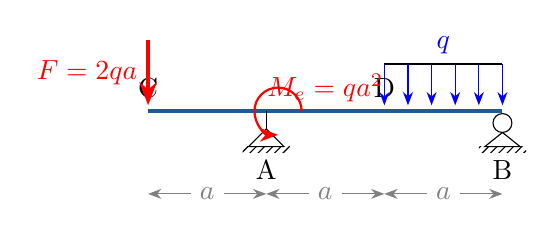
\begin{tikzpicture}[scale=1.5, >=Stealth]
    % Draw beam
    \draw[ultra thick, accent] (0,0) -- (3,0);
    
    % Draw supports
    \draw (1,-0.15) -- (1,0);
    \draw (1,-0.15) -- (0.85,-0.3) -- (1.15,-0.3) -- cycle;
    \pattern[pattern=north east lines] (0.8,-0.35) rectangle (1.2,-0.3);
    \node at (1,-0.5) {A};
    
    \draw (3,-0.1) circle (0.08);
    \draw (3,-0.18) -- (2.85,-0.3) -- (3.15,-0.3) -- cycle;
    \pattern[pattern=north east lines] (2.8,-0.35) rectangle (3.2,-0.3);
    \node at (3,-0.5) {B};
    
    \node at (0,0.2) {C};
    \node at (2,0.2) {D};
    
    % Dimensions
    \draw[<->, gray] (0,-0.7) -- node[fill=white] {$a$} (1,-0.7);
    \draw[<->, gray] (1,-0.7) -- node[fill=white] {$a$} (2,-0.7);
    \draw[<->, gray] (2,-0.7) -- node[fill=white] {$a$} (3,-0.7);
    
    % Load F at C
    \draw[->, red, very thick] (0,0.6) -- node[left] {$F=2qa$} (0,0.05);
    
    % Moment Me at A
    \draw[->, red, thick] (1.3,0) arc (0:270:0.2);
    \node[red] at (1.5,0.2) {$M_e = qa^2$};
    
    % Distributed load on DB
    \draw[thick] (2,0.4) -- (3,0.4);
    \foreach \x in {2.0,2.2,2.4,2.6,2.8,3.0} {
        \draw[->, blue, thin] (\x,0.4) -- (\x,0.05);
    }
    \node[blue, above] at (2.5,0.4) {$q$};
\end{tikzpicture}
\end{center}

\subsubsection*{解答：}

\textbf{（1）A、B处的约束反力}

设定支座反力 $R_A, R_B$ 竖直向上。根据静力平衡条件：
\begin{itemize}
    \item 竖直方向力平衡：
    \[
        \sum Y = 0 \implies R_A + R_B - F - q \cdot a = 0 \implies R_A + R_B = 3qa
    \]
    \item 对A点取矩平衡：
    \[
        \sum M_A = 0 \implies F \cdot a - M_e - q \cdot a \cdot 1.5a + R_B \cdot 2a = 0
    \]
    代入已知条件 $F = 2qa, M_e = qa^2$:
    \[
        2qa^2 - qa^2 - 1.5qa^2 + 2a R_B = 0 \implies -0.5qa^2 + 2a R_B = 0 \implies R_B = \frac{1}{4}qa = 0.25qa
    \]
    \item 从而求得 A 处的反力为：
    \[
        R_A = 3qa - 0.25qa = \frac{11}{4}qa = 2.75qa
    \]
\end{itemize}

\textbf{（2）梁的剪力图与弯矩图}

根据内力方程进行绘图：
\begin{itemize}
    \item \textbf{CA 段} ($x \in [0, a)$):
    \[
        Q(x) = -F = -2qa, \quad M(x) = -F \cdot x = -2qa x
    \]
    在 $x=a$ 的左侧，$M(a^-) = -2qa^2$。
    \item \textbf{AD 段} ($x \in (a, 2a)$):
    \[
        Q(x) = -F + R_A = -2qa + 2.75qa = 0.75qa
    \]
    由于 A 点作用顺时针集中弯矩 $M_e = qa^2$，弯矩图在 A 点发生突变：
    \[
        M(a^+) = M(a^-) + M_e = -2qa^2 + qa^2 = -qa^2
    \]
    AD 段弯矩方程为：
    \[
        M(x) = -2qa^2 + 2.75qa(x-a) + qa^2 = 0.75qa(x-a) - qa^2
    \]
    在 $x=2a$ （D点）：
    \[
        M(2a) = 0.75qa^2 - qa^2 = -0.25qa^2
    \]
    \item \textbf{DB 段} ($x \in (2a, 3a)$):
    \[
        Q(x) = 0.75qa - q(x-2a)
    \]
    剪力为零的位置（$Q(x_0) = 0$）：
    \[
        0.75qa - q(x_0-2a) = 0 \implies x_0 = 2.75a
    \]
    弯矩方程为：
    \[
        M(x) = -0.25qa^2 + 0.75qa(x-2a) - \frac{1}{2}q(x-2a)^2
    \]
    在 $x_0 = 2.75a$ 处弯矩达到最大值：
    \[
        M(2.75a) = -0.25qa^2 + 0.75qa(0.75a) - 0.5q(0.75a)^2 = 0.03125 qa^2 = \frac{1}{32}qa^2
    \]
\end{itemize}

\begin{center}
\begin{tikzpicture}[scale=1.5, >=Stealth]
    % Shear Force Diagram Q
    \draw[axisgray, ->] (-0.2,0) -- (3.5,0) node[right] {$Q$};
    \draw[ultra thick, red] (0,-1) -- (1,-1);
    \draw[red, dashed] (1,-1) -- (1,0.375);
    \draw[ultra thick, red] (1,0.375) -- (2,0.375);
    \draw[ultra thick, red] (2,0.375) -- (3,-0.125);
    \draw[red, dashed] (3,-0.125) -- (3,0);
    \node[left, red] at (0,-1) {$-2qa$};
    \node[above, red] at (1.5,0.375) {$0.75qa$};
    \node[below, red] at (3,-0.125) {$-0.25qa$};
    \node[above] at (1.5,0.8) {剪力图 $Q(x)$};
\end{tikzpicture}
\end{center}

\begin{center}
\begin{tikzpicture}[scale=1.5, >=Stealth]
    % Bending Moment Diagram M
    \draw[axisgray, ->] (-0.2,0) -- (3.5,0) node[right] {$M$};
    \draw[ultra thick, blue] (0,0) -- (1,-2);
    \draw[blue, dashed] (1,-2) -- (1,-1);
    \draw[ultra thick, blue] (1,-1) -- (2,-0.25);
    \draw[ultra thick, blue, domain=2:3, samples=20] plot (\x, {-0.25 + 0.75*(\x-2) - 0.5*(\x-2)^2});
    \node[below, blue] at (1,-2) {$-2qa^2$};
    \node[above, blue] at (1,-1) {$-qa^2$};
    \node[below, blue] at (2,-0.25) {$-0.25qa^2$};
    \node[above, blue] at (2.75,0.03125) {$\frac{1}{32}qa^2$};
    \node[above] at (1.5,0.5) {弯矩图 $M(x)$};
\end{tikzpicture}
\end{center}

\textbf{（3）最大内力及其位置}
\begin{itemize}
    \item 最大剪力：$|Q|_{\max} = 2qa$，发生于 \textbf{CA 段全截面}。
    \item 最大弯矩：$|M|_{\max} = 2qa^2$（绝对值），发生于 \textbf{支座 A 的左侧截面}。
\end{itemize}

\newpage

\section*{二、薄壁截面切应力流方向分析}

\textbf{2、如下图为承受横向载荷的梁的横截面。若剪力均为铅垂向下，试画出各截面上的切应力流方向。}

\begin{center}
\begin{tikzpicture}[scale=1.2]
    % (a) Double-U shape
    \draw[ultra thick] (0,1.5) -- (0,0) -- (0.8,0) -- (0.8,1.5);
    \draw[ultra thick] (0.8,0) -- (1.6,0) -- (1.6,1.5);
    \node at (0.8,-0.5) {(a) 双 U 截面};
    
    % Flow arrows for (a)
    \draw[->, red, thick] (0,1.2) -- (0,0.6);
    \draw[->, red, thick] (0.8,1.2) -- (0.8,0.6);
    \draw[->, red, thick] (1.6,1.2) -- (1.6,0.6);
    \draw[->, red, thick] (0.2,0) -- (0.6,0);
    \draw[->, red, thick] (1.4,0) -- (1.0,0);
    
    % (b) E-shape
    \begin{scope}[xshift=4cm]
        \draw[ultra thick] (1.5,1.5) -- (0,1.5) -- (0,-0.5) -- (1.5,-0.5);
        \draw[ultra thick] (0,0.5) -- (1.5,0.5);
        \node at (0.75,-1.0) {(b) E 形截面};
        
        % Flow arrows for (b)
        \draw[->, red, thick] (1.2,1.5) -- (0.6,1.5);
        \draw[->, red, thick] (0,1.2) -- (0,0.8);
        \draw[->, red, thick] (0.6,0.5) -- (1.2,0.5);
        \draw[->, red, thick] (0,0.2) -- (0,-0.2);
        \draw[->, red, thick] (0.6,-0.5) -- (1.2,-0.5);
    \end{scope}
\end{tikzpicture}
\end{center}

\subsubsection*{设计原则与流向分析：}
切应力流的计算公式为 $q = \frac{V Q_z}{I_z}$。
\begin{itemize}
    \item 对于自由边缘，$Q_z = 0$，应力流为零，以此为起点。
    \item 竖直腹板承受主要剪力，其上的应力流应向下（与剪力 $V$ 方向一致）。
    \item 翼缘与腹板交界处必须满足节点处的应力流连续性（流体守恒条件）。
\end{itemize}
\textbf{流向说明}：
\begin{itemize}
    \item \textbf{双 U 截面}：外侧两竖直边和中间竖直边顶端为自由端，应力流从三根立柱向下流动，在底板处相向汇合。
    \item \textbf{E 形截面}：应力流从上、下两片横梁向左流向竖直腹板，再沿竖直腹板向下流，在中间横梁处向右流出，符合应力平衡与对称性要求。
\end{itemize}

\newpage

\section*{三、斜截面应力分析}

\textbf{3、已知通过一点的两个斜截面 $n_1$，$n_2$ 上的应力为 $\sigma_{\alpha 1}=52.3\text{ MPa}$、$\tau_{\alpha 1}=-18.6\text{ MPa}$，$\sigma_{\alpha 2}=20\text{ MPa}$、$\tau_{\alpha 2}=-10\text{ MPa}$，试用应力圆求：（1）$n_1$、$n_2$ 面的夹角 $\alpha$；（2）该点的主应力及主平面位置。}

\subsubsection*{解答：}

\textbf{（1）确定应力圆基本参数}

应力圆方程为 $(\sigma - \sigma_0)^2 + \tau^2 = R^2$。将两斜截面上的应力点 $P_1(52.3, -18.6)$ 和 $P_2(20, -10)$ 代入方程：
\[
    (52.3 - \sigma_0)^2 + (-18.6)^2 = R^2
\]
\[
    (20 - \sigma_0)^2 + (-10)^2 = R^2
\]
联立求得：
\[
    (52.3 - \sigma_0)^2 + 345.96 = (20 - \sigma_0)^2 + 100
\]
\[
    2735.29 - 104.6 \sigma_0 + 345.96 = 400 - 40 \sigma_0 + 100
\]
\[
    2581.25 = 64.6 \sigma_0 \implies \sigma_0 = 39.96\text{ MPa} \approx 40\text{ MPa}
\]
将 $\sigma_0 = 40\text{ MPa}$ 代入求半径 $R$：
\[
    R^2 = (20 - 40)^2 + 100 = 500 \implies R = 10\sqrt{5} \approx 22.36\text{ MPa}
\]

\textbf{（2）求夹角 $\alpha$}

在应力圆上，$P_1$ 和 $P_2$ 点对应的旋转角为 $2\alpha$：
\[
    \tan(2\alpha_1) = \frac{-18.6}{52.3 - 40} = -1.512 \implies 2\alpha_1 = -56.5^\circ
\]
\[
    \tan(2\alpha_2) = \frac{-10}{20 - 40} = 0.5
\]
由于 $P_2$ 处的剪应力为负，且法向应力小于圆心应力，所以在应力圆中 $P_2$ 处于第三象限：
\[
    2\alpha_2 = -180^\circ + 26.6^\circ = -153.4^\circ
\]
两点在应力圆上的角度差为：
\[
    \Delta \theta = 2\alpha = |(-56.5^\circ) - (-153.4^\circ)| = 96.9^\circ \implies \alpha \approx 48.45^\circ
\]

\textbf{（3）主应力及主平面}
\begin{itemize}
    \item 第一主应力：$\sigma_1 = \sigma_0 + R = 40 + 22.36 = 62.36\text{ MPa}$
    \item 第二主应力：$\sigma_2 = \sigma_0 - R = 40 - 22.36 = 17.64\text{ MPa}$
    \item 主平面位置：主平面与 $n_1$ 面的夹角为 $\alpha_p = \frac{56.5^\circ}{2} = 28.25^\circ$。
\end{itemize}

\newpage

\section*{四、压杆稳定与刚度设计题}

\textbf{4、一端固支的横梁（AB）上作用了垂直向下的均匀分布载荷 $q$，梁端部 B 受到向下的集中载荷 $qa$，在梁 AB 的中点 C 处有一铅垂杆 CD 铰接，CD 杆的 D 点与地面铰支固定。若 AB 梁长为 $2a$，CD 杆长为 $L$。已知横梁和立柱的弹性模量分别为 $E_1$ 和 $E_2$，假设立柱属于大柔度杆弹性失稳，AB 和 CD 均为圆形截面，半径为 $R$。如果结构的破坏为失稳破坏，计算临界载荷集度 $q_{\text{cr}}$。}

\subsubsection*{解答：}

\textbf{（1）变形协调分析与 CD 杆受力}

设 CD 杆的受压轴力为 $F_{\text{CD}}$。梁在 C 点处的挠度为 $w_C$。由于 D 端固定铰支，C 端与梁铰接，CD 杆的缩短量为：
\[
    \Delta_L = \frac{F_{\text{CD}} L}{E_2 (\pi R^2)}
\]
根据变形协调条件，C 点处的挠度 $w_C$ 等于立柱的缩短量 $\Delta_L$。对于大柔度杆，立柱的轴向收缩极小，可近似近似为刚性支座（即 $w_C = 0$）。

利用静不定叠加法计算梁在 C 处的挠度：
\begin{itemize}
    \item 均布载荷 $q$ 引起的 C 点（距固支端 $a$）弯曲挠度为：
    \[
        w_{C, q} = \frac{q a^4}{24 E_1 I_1} \left( 1 + 24 - 8 \right) = \frac{17 q a^4}{24 E_1 I_1}
    \]
    \item 端部集中力 $F_B = qa$ 引起的 C 点挠度为：
    \[
        w_{C, P} = \frac{qa \cdot a^2}{6 E_1 I_1}(6a - a) = \frac{20 q a^4}{24 E_1 I_1}
    \]
    \item 支撑力 $F_{\text{CD}}$ 引起的 C 点反向挠度为：
    \[
        w_{C, F} = -\frac{F_{\text{CD}} a^3}{3 E_1 I_1} = -\frac{8 F_{\text{CD}} a^3}{24 E_1 I_1}
    \]
\end{itemize}
令 $w_C = 0 \implies 17qa^4 + 20qa^4 - 8 F_{\text{CD}} a^3 = 0 \implies F_{\text{CD}} = \frac{37}{8}qa = 4.625 qa$。

\textbf{（2）CD 杆的临界屈服载荷}

根据 Euler 临界载荷公式，两端铰支压杆（$\mu=1$）的临界载荷为：
\[
    P_{\text{cr}} = \frac{\pi^2 E_2 I_2}{L^2} = \frac{\pi^2 E_2 (\pi R^4 / 4)}{L^2} = \frac{\pi^3 E_2 R^4}{4 L^2}
\]

\textbf{（3）临界载荷集度 $q_{\text{cr}}$}

当 $F_{\text{CD}} = P_{\text{cr}}$ 时，立柱发生失稳破坏：
\[
    \frac{37}{8} q_{\text{cr}} a = \frac{\pi^3 E_2 R^4}{4 L^2} \implies q_{\text{cr}} = \frac{2 \pi^3 E_2 R^4}{37 a L^2}
\]

\newpage

\section*{五、双材料组合悬臂梁分析题}

\textbf{5、悬臂梁由两种材料不同、尺寸完全相同的矩形截面粘接而成。已知弹性模量 $E_1=2E_2$，矩形截面宽为 $b$，高为 $h$，梁长为 $l$。}\\
\textbf{（1）当轴向力 $F_{\text{p}}$ 的作用线与二杆的组合轴线 $OO_1$ （粘合缝）一致时，悬臂梁会发生什么样的变形？}\\
\textbf{（2）力 $F_{\text{p}}$ 作用在哪里时，梁的端截面仅发生水平方向移动，而不发生转动？}

\subsubsection*{解答：}

\textbf{（1）$F_{\text{p}}$ 作用于 $OO_1$ 时的变形分析}

当轴向力作用于界面时，由于两种材料的刚度不同，截面上的中性轴并不在几何中心（粘缝处）。
我们计算截面的物理等效形心（即拉伸中心）的位置 $y_c$：
设定粘缝 $OO_1$ 处为 $y=0$，上方为材料 1（$E_1=2E_2$），下方为材料 2（$E_2$）：
\[
    y_c = \frac{\int E y \diff A}{\int E \diff A} = \frac{E_1 \cdot b \int_{0}^h y \diff y + E_2 \cdot b \int_{-h}^0 y \diff y}{E_1 (bh) + E_2 (bh)} = \frac{2 E_2 \cdot \frac{h^2}{2} - E_2 \cdot \frac{h^2}{2}}{3 E_2 h} = \frac{h}{6}
\]
这说明，等效拉伸中心在粘缝上方 $\frac{h}{6}$ 处。
当外力 $F_{\text{p}}$ 作用于 $OO_1$（$y=0$）时，产生偏心矩 $e = -h/6$，这等效于一个轴向拉力和弯矩 $M = -F_{\text{p}} \cdot \frac{h}{6}$ 的共同作用。
因此，\textbf{悬臂梁会发生拉伸与向下弯曲的组合变形}。

\textbf{（2）使端截面无转动的力作用点}

要使端截面只产生水平拉伸而不发生转动，轴向外力 $F_{\text{p}}$ 必须作用在复合截面的等效形心（拉伸中心）上。
即外力 $F_{\text{p}}$ 应作用在：\textbf{粘缝 $OO_1$ 上方 $\frac{h}{6}$ 处（即处于材料 1 内部）}。

\newpage

\section*{六、并联圆轴与圆管的扭转分析}

\textbf{6、一圆管套在一个圆轴外，两端焊住，如下图所示。圆轴和圆管的切变模量分别为 $G_1, G_2$，圆轴外径为 $D$，内径为 $d$（为中空圆轴），圆管外径为 $d_1$，内径为 $D$（紧密套接）。当两端共同施加扭矩 $M_x$ 时，求圆管和圆轴各自承担的扭矩。}

\subsubsection*{解答：}

根据扭转变形协调条件，圆管（2）和圆轴（1）由于两端焊接，其扭转角必须相等：
\[
    \theta_1 = \theta_2 = \theta
\]
根据圆截面扭转公式，两部分分担的扭矩分别为：
\[
    T_1 = G_1 I_{p1} \theta, \quad T_2 = G_2 I_{p2} \theta
\]
其中 polar moment of inertia 极惯性矩分别为：
\[
    I_{p1} = \frac{\pi}{32}(D^4 - d^4), \quad I_{p2} = \frac{\pi}{32}(d_1^4 - D^4)
\]
由平衡条件 $T_1 + T_2 = M_x$：
\[
    (G_1 I_{p1} + G_2 I_{p2}) \theta = M_x \implies \theta = \frac{M_x}{G_1 I_{p1} + G_2 I_{p2}}
\]
由此求得各自承担的扭矩为：
\[
    T_1 = \frac{G_1 I_{p1}}{G_1 I_{p1} + G_2 I_{p2}} M_x, \quad T_2 = \frac{G_2 I_{p2}}{G_1 I_{p1} + G_2 I_{p2}} M_x
\]

\end{document}
